%% Background Theory
%%=========================================

\chapter{Background Theory}
\label{ch:background}
In this chapter we introduce the background theory relevant to the related work presented in the Chapter \ref{ch:related_work}. Feedforward neural networks are introduced in Section \ref{sec:feedforward_neural_network}. Recurrent neural networks, and some common recurrent neural network architectures, are introduced in Section \ref{sec:reccurent_neural_network}. The encoder-decoder framework is introduced in Section \ref{sec:encoder-decoder}, and two types of vocabulary encoding methods are presented in Section \ref{sec:vocabulary_encoding}.

%%=========================================

\section{Feedforward Neural Network}
\label{sec:feedforward_neural_network}
Artificial neural network is a computational model used in machine learning and computer science. The idea behind neural networks lies in the use of artificial neurons, an idea that can be traced back to the 1940s. These artificial neurons are loosely analogous to axons in a biological brain, and artificial neural networks is an attempt at modeling the information process capabilities of nervous systems \citep{russell2010aimodernapproach}.

\begin{figure}[ht]
    \centering
    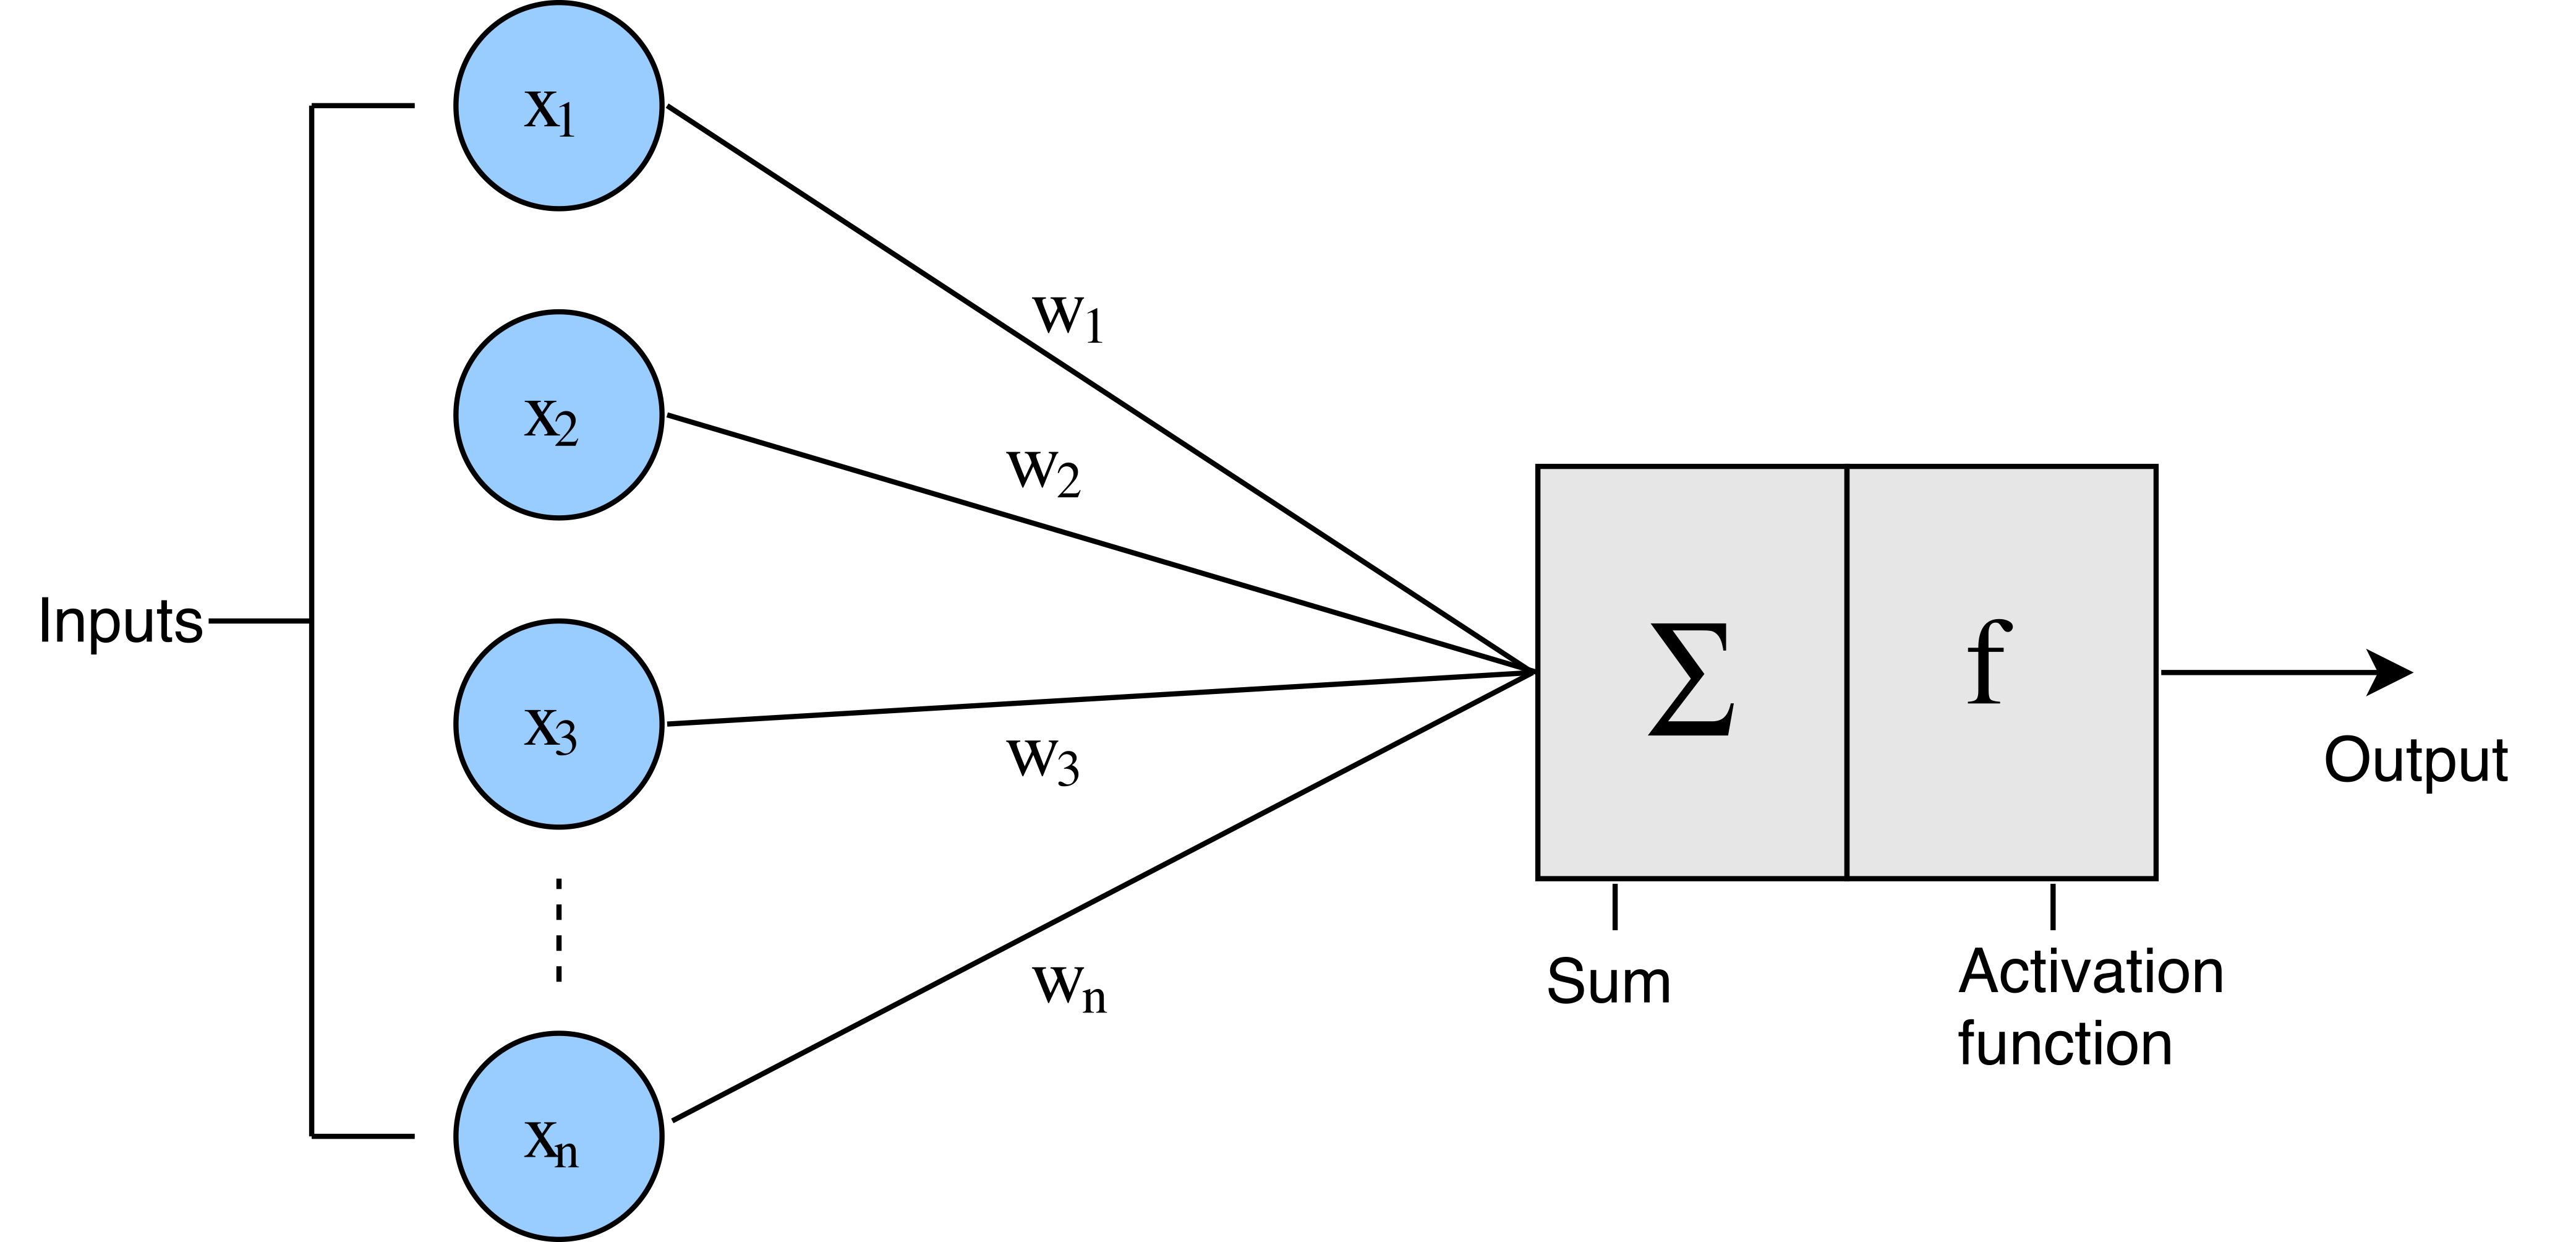
\includegraphics[width=1\textwidth]{fig/related_work/perceptron.png}
    \caption{Illustration of a mathematical model of a neuron}
    \label{fig:nn-perceptron}
\end{figure}

Figure \ref{fig:nn-rnn} illustrates a simple mathematical model for a neuron, often called a unit or a node. This unit ``fires'' when a linear combination of its inputs exceeds some threshold. A neural network is a collection of many such units. The properties of a network are determined by its topology, as well as the properties of the units. Networks are constructed by directly linking nodes with each other. A link from unit \(i\) to unit \(j\) serves to propagate the activation \(a_{i}\) from \(i\) to \(j\). The strength and sign of the signal are determined by the numeric weight that is associated with the unit. 

A feedforward network consists of units which have connections that only goes in one direction. These node receives input from the ``upstream'' nodes, and delivers output to the ``downstream'' nodes, forming a directed acyclic graph \citep{russell2010aimodernapproach}.

%%=========================================

\section{Recurrent Neural Network}
\label{sec:reccurent_neural_network}
A recurrent neural network (RNN) is a type of artificial neural network. This type of neural networks creates an internal state of the network which allows it to express dynamic temporal behavior. The structure of a recurrent neural network is much like a feedforward network, but in addition to feeding ``downstream'' nodes, nodes also feed its output back into its own inputs. This type of architecture can support a short-term memory, a feature that is necessary in problems where input depends on previous input \citep{russell2010aimodernapproach}, for example in areas such as speech recognition.

\begin{figure}[ht]
    \centering
    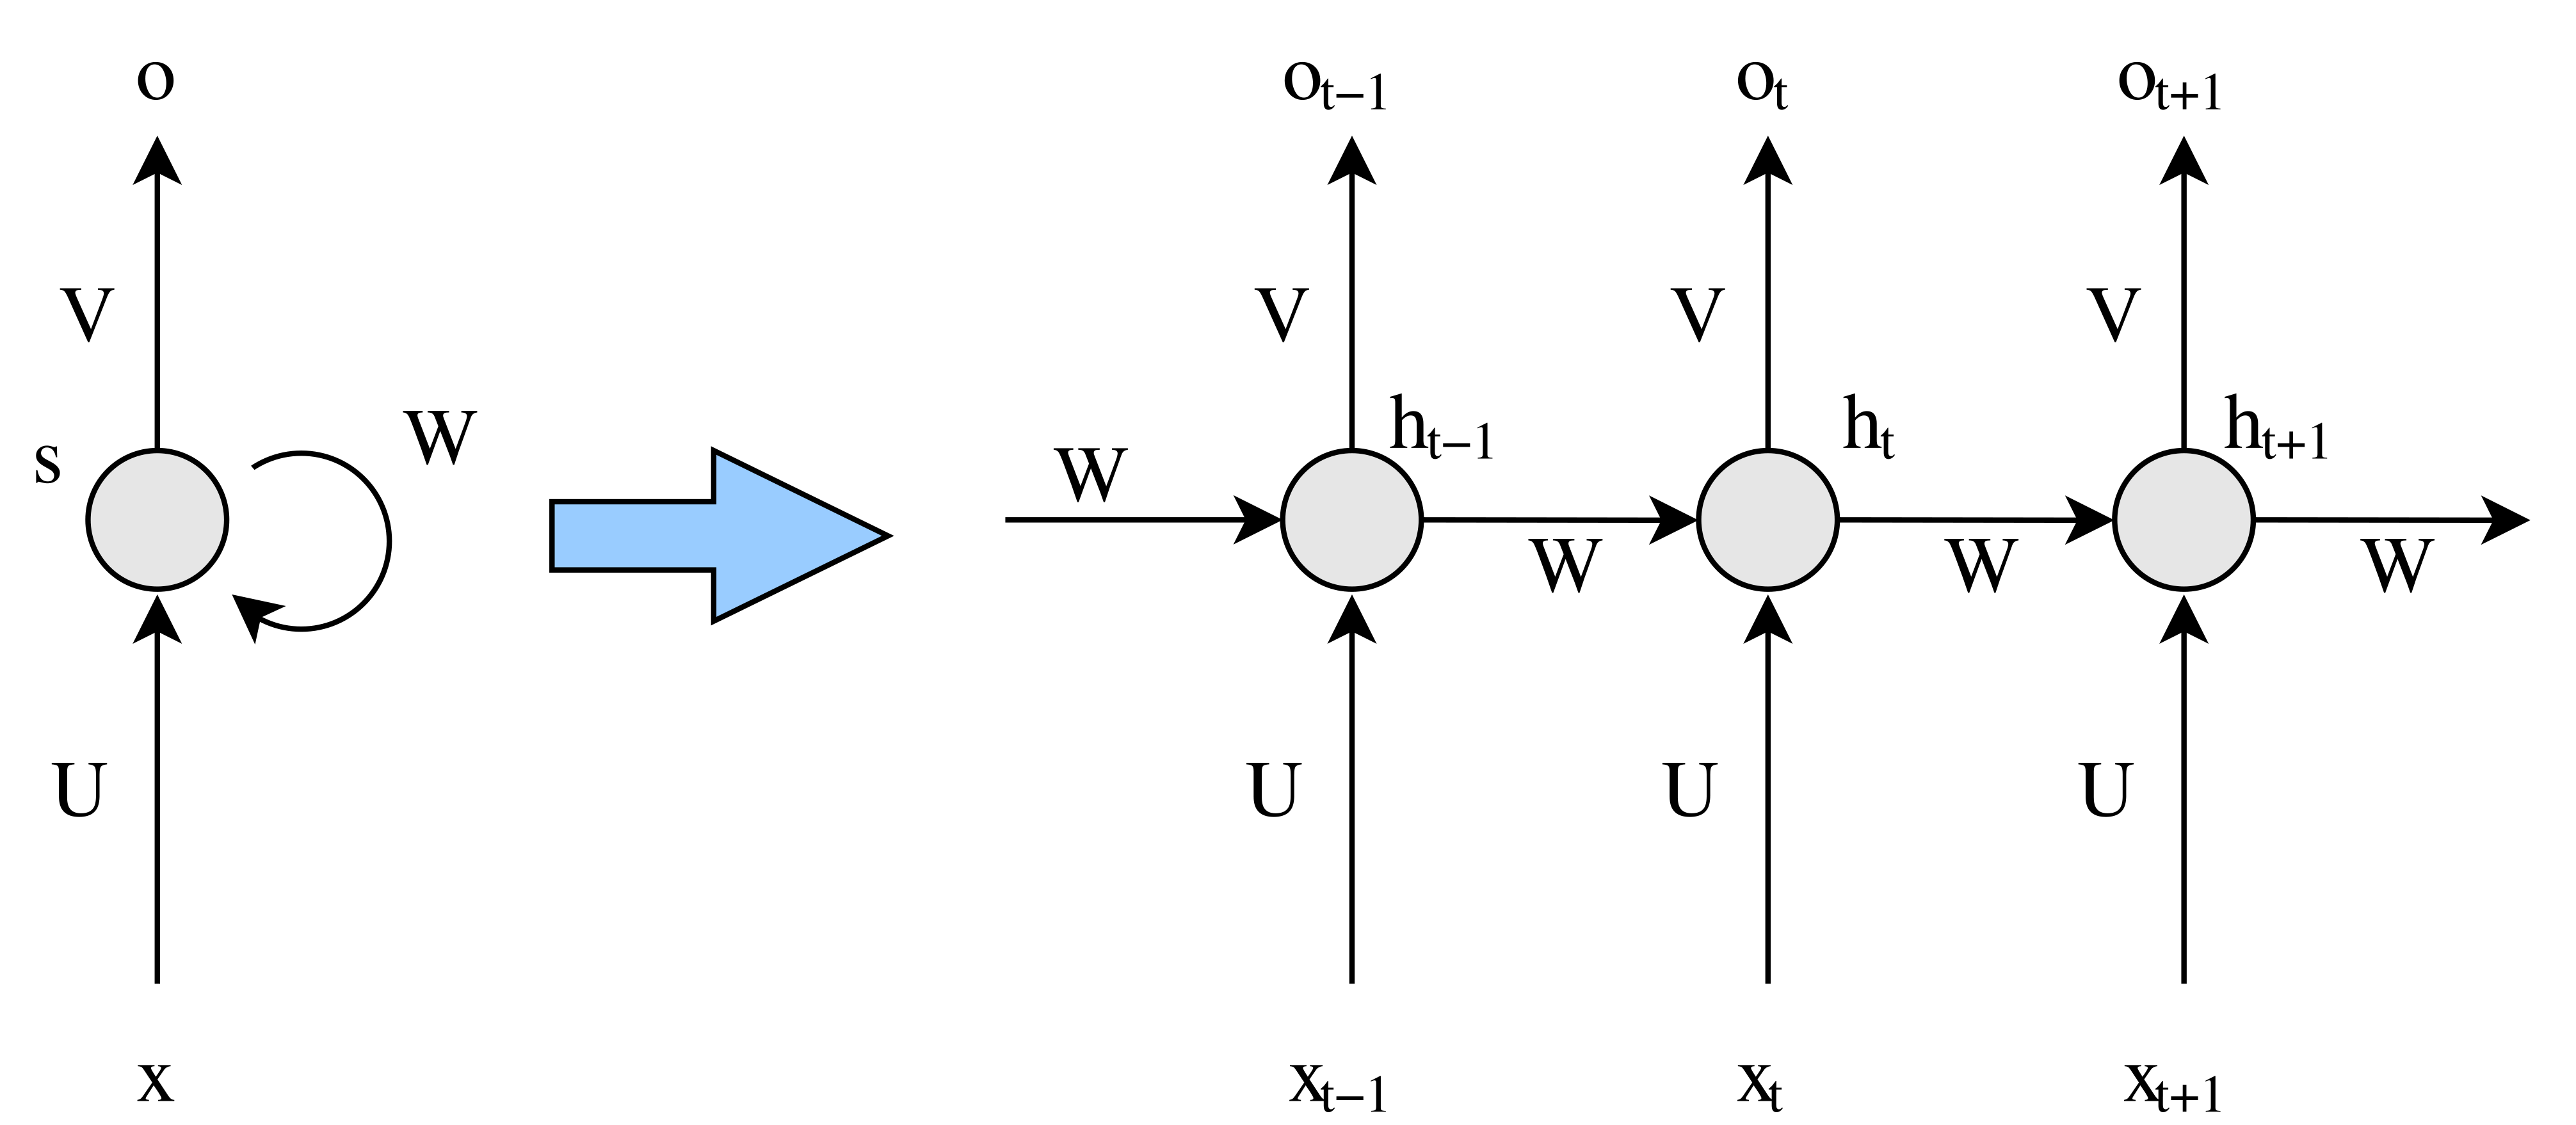
\includegraphics[width=0.8\textwidth]{fig/related_work/nn_recurrent.png}
    \caption{A compact and an unfolded recurrent neural network}
    \label{fig:nn-rnn}
\end{figure}

We can consider recurrent neural networks as a loop, and we can unfold it into a complete sequence, as illustrated in Figure \ref{fig:nn-rnn}. In the figure, \(X_{t}\) is the input, and \(h_{t}\) is the hidden state of the recurrent network at timestep \(t\). The hidden state function as the unit's memory. The hidden state from timestep \(t\) is reused in the next timestep \(t+1\), along with the input of the current timestep. It is also important to note that the network shares the same weights \(W\) across several timesteps. The recurrent neural network has input to hidden connections parametrized by a weight matrix \(U\), as well as hidden-to-hidden recurrent connections parametrized by a weight matrix \(W\). In addition, the network has hidden-to-output connection parametrized by a weight matrix \(V\) \citep{goodfellow2016deeplearning}.

\begin{align}
    \begin{split}\label{eq:rnn-eq-1}
        h_{t}&=\sigma(b+Wh_{t-1}+Ux_{t})
    \end{split}\\
    \begin{split}\label{eq:rnn-eq-2}
        \hat{y_{t}}&=\sigma(c+Vh_{t})
    \end{split}
\end{align}

Equations \ref{eq:rnn-eq-1} and \ref{eq:rnn-eq-2} are slightly simplified from \cite{goodfellow2016deeplearning}, and defines the forward propagation of the model illustrated in Figure \ref{fig:nn-rnn}. The parameters \(b\) and \(c\) are the bias vectors. Computing the gradient in a recurrent neural network can be done with an iterative gradient descent back-propagation algorithm such as back-propagation through time \citep{werbos1990backpropagation, rumelhart1988learning}. 

\subsection{Input and Output Shapes}
\label{sec:input_and_output_shapes}
Recurrent neural networks are usually fed data that has an input shape of {\tt (timesteps, features)}, where the first dimension defines how many timesteps our data consists of, and the last dimension defines the number of features for each timestep. Table \ref{table:temporal_weather_data} contains weather data for Trondheim in Norway in the period June 2016 to September 2016\footnote{\url{https://www.yr.no/sted/Norge/Sør-Trøndelag/Trondheim/Trondheim/statistikk.html}}. This example has a total of four timesteps, one for each month in the period, and a total of three separate features: temperature, rain, and wind. This data would have an input shape of {\tt (4, 3)}. We can consider this data as recording a total of three features over the course of four timesteps.

\begin{table}[H]
    \centering
    \begin{tabular}{|l|l|l|l|l|}
        \hline
        \multirow{2}{*}{\textbf{Features}}   & \multicolumn{3}{c}{\textbf{Timesteps}}                                   &                        \\ \cline{2-5}
                                             & \textbf{1}             & \textbf{2}             & \textbf{3}             & \textbf{4}             \\ \hline
        Temperature (average)                & 12.2\textdegree        & 14.8\textdegree        & 13.0\textdegree        & 12.2\textdegree        \\ \hline
        Rain (total)                         & 31.7 mm                & 77.5 mm                & 87.1 mm                & 77.6 mm                \\ \hline
        Wind (average)                       & 2.3 m/s                & 2.0 m/s                & 2.1 m/s                & 1.9 m/s                \\ \hline
    \end{tabular}
    \caption{Weather data over time}
    \label{table:temporal_weather_data}
\end{table}

The output of a typical recurrent neural network has a shape of {\tt (units)}, where {\tt units} is the number of output units in the network. Considering the compact network in Figure \ref{fig:nn-rnn}, the output of a recurrent neural network is the output of the last iteration of the loop. One may also use the output of every iteration in the loop, which results in an output shape of {\tt (timesteps, units)}, where the dimensionality of the timesteps in the output is equal to the dimensionality of the timesteps in the input.

\subsection{Long-Short Term Memory}
\label{sec:long_short_term_memory}
Long-Short Term Memory (LSTM) is a recurrent neural network architecture. It was first proposed by \cite{hochreiter1997long} and was meant to address some of the shortcomings of more basic recurrent neural network architectures. \cite{bengio1994learning} showed that recurrent neural networks faced an increasingly difficult problem as the duration of the dependencies to be captured were increased. While the architecture could take into account short-term dependencies rather well, long-term dependencies were increasingly difficult to learn. The LSTMs were explicitly designed to avoid the long-term dependency problem. 

\begin{figure}[ht]
    \centering
    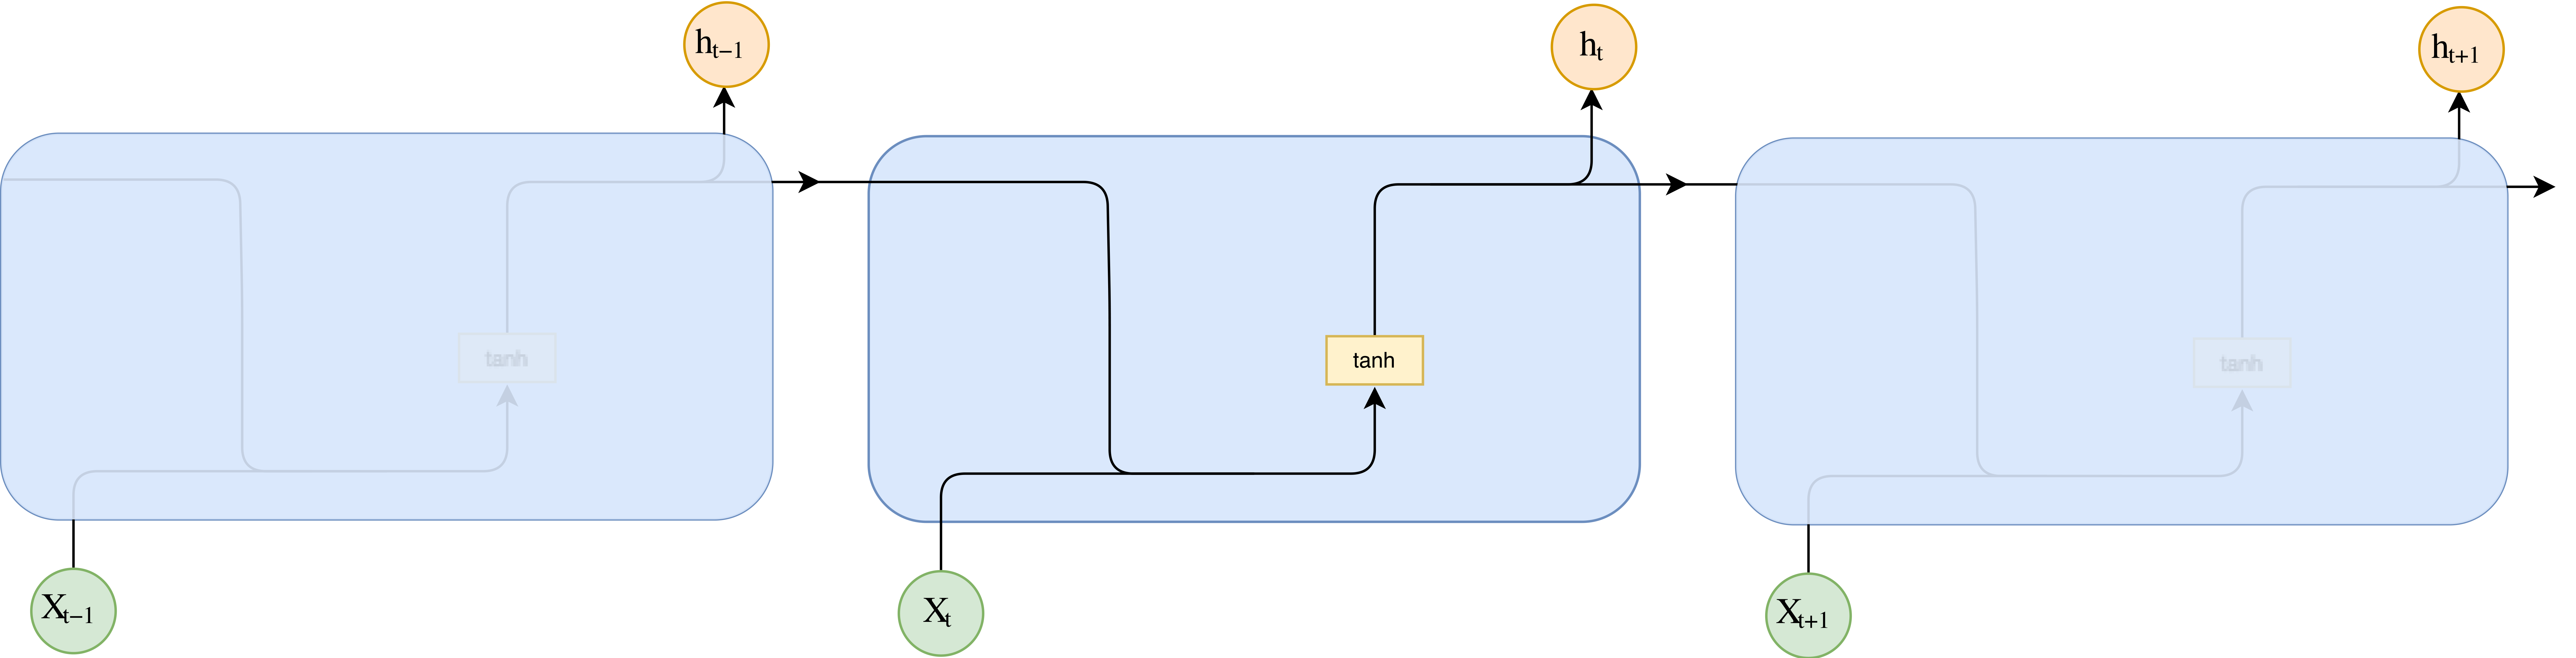
\includegraphics[width=1\textwidth]{fig/related_work/rnn_flow.png}
    \caption{Flow of a standard recurrent neural network}
    \label{fig:nn-rnn-flow}
\end{figure}

Figure \ref{fig:nn-rnn-flow} illustrates the chain like structure of a standard recurrent neural network. Its architecture is relatively simple, containing only one layer. In this illustration, the layer uses the hyperbolic tangent function (tanh) as its activation function.

\begin{figure}[ht]
    \centering
    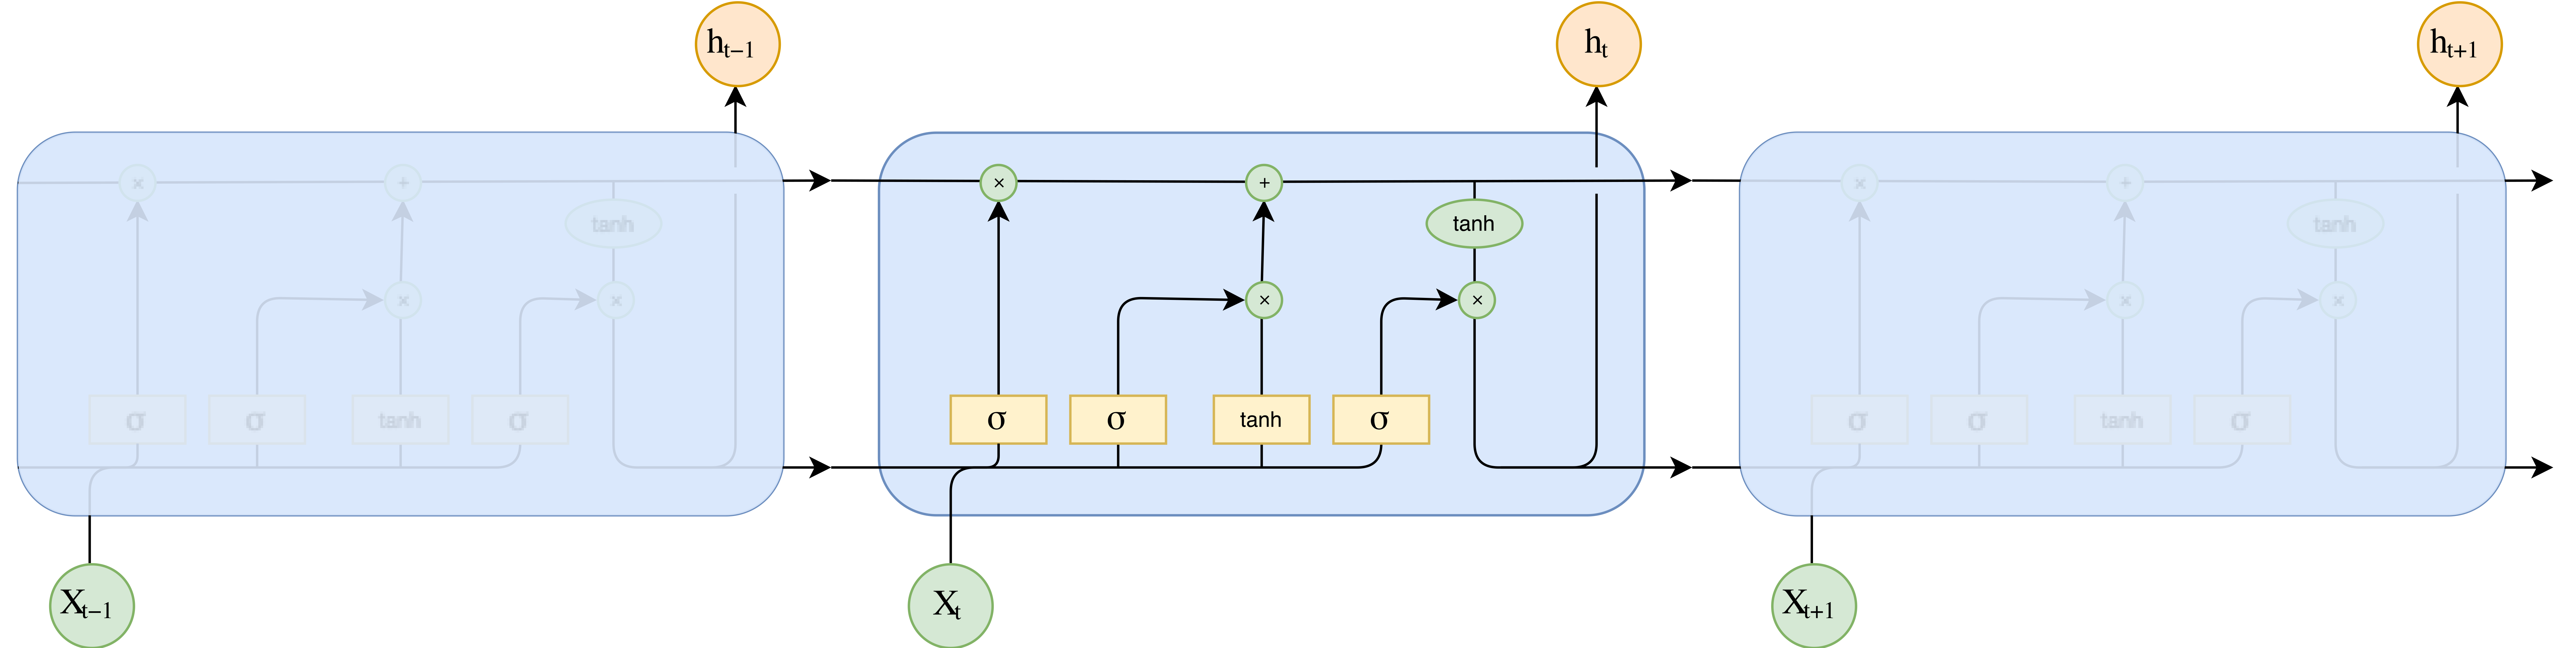
\includegraphics[width=1\textwidth]{fig/related_work/lstm_flow.png}
    \caption{Flow of an LSTM cell}
    \label{fig:nn-lstm-flow}
\end{figure}

Figure \ref{fig:nn-lstm-flow} illustrates a similar chain structure, but that of an LSTM cell. The LSTM module has a total of four neural network layers, whereas the simpler recurrent neural network only has one. The topmost horizontal line carries the cell state of the unit, while the horizontal line at the bottom carries the hidden state of the unit. The LSTM unit is enriched by several so-called gating units. These gates regulate what information is remembered by the cell state, and what is forgotten. The leftmost sigmoid layer is called the ``forget gate layer''. This gate decides what the state should forget from the existing information. The next sigmoid gate is called the ``input gate layer'' and determines which values should be updated. The hyperbolic tangent gate layer creates a vector of candidate values, which could be added to the cell state. After the state is updated, or the candidate is thrown away, the final sigmoid gate, the ``output gate layer'', decides which parts of the cell state should be outputted \citep{hochreiter1997long, goodfellow2016deeplearning, olah2015lstm, gers2002learning}. The first proposed version of the LSTM did not have a forget gate. It was introduced by \cite{gers2000learning} and allowed the LSTM to reset its state. This version has since become one of the most common variants of the LSTM.

\subsubsection{Variants of LSTM}
The LSTM implementation described above is one of the traditional LSTMs. There exist other variants of the architecture with other characteristics. One popular LSTM variant was introduced by \cite{gers2001lstm}. Their variant added ``peephole'' connections. These connections allow the gate layer to look at the cell state. The idea behind this variant was to have an LSTM that could learn to selectively reset its memory contents, and in turn, produce stable results in the presence of never-ending input streams. \cite{gers2001lstm} stated that their LSTM variant with peephole connections and forget gates were clearly superior to the traditional LSTM. 

Another variant is the ``Convolutional LSTM'', proposed by \cite{xingjian2015convolutional}. Their variant extended the traditional LSTM and added convolutional structures to both the input-to-state and state-to-state transitions. Their conclusion was that their proposed ``ConvLSTM'' layer was suitable for spatiotemporal data due to its inherent convolutional structure.

A comparison of various LSTM variants was carried out by \cite{greff2016lstm}. They concluded that the traditional, vanilla LSTM, performed reasonable well on various datasets. They investigated a total of eight variants of the LSTM, and in their experiments, none of the eight modifications significantly improved performance. However, certain modifications simplified the LSTMs without significantly decreasing performance. 

\subsection{GRU}
Another popular modification of the LSTM was proposed by \cite{chung2014empirical}. Their simplified variant called the Gated Recurrent Unit, or GRU for short, uses neither peepholes nor output activation functions. Instead, the GRU couples the input and the forget gate into an update gate. The GRU also merges the hidden and cell states  \citep{greff2016lstm, chung2014empirical}. Comparisons between the LSTM and the GRU units have shown mixed results, and experiments have concluded that there is no clear winner between the two \citep{greff2016lstm, chung2014empirical}. \cite{jozefowicz2015empirical} compared various LSTM and GRU units and reported that GRUs outperformed the LSTM on all tasks except language modeling.

%%=========================================

\section{Encoder-Decoder Models}
\label{sec:encoder-decoder}
The encoder-decoder framework is a concept centralized around two recurrent neural networks. The idea is to encode the input in the first neural network and decode it in the second network. The first recurrent neural network, also called the encoder, reads the input sentence, a sequence of vectors \(X = (x_{1}, x_{2}, \ldots, x_{n})\). This sequence is then encoded into a vector \(c\), which may or may not be of fixed length \citep{sutskever2014sequence, cho2014learning}. 

The decoder is often trained to predict the next word \(y_{t'}\) given the context vector \(c\) and all the previously predicted words \({y_1, \ldots, y_{t'-1}}\). \cite{bahdanau2014neural} summarizes the architecture with:

\begin{quote}
    The decoder defines a probability over the translation \(y\) by decomposing the joint probability into the ordered conditionals:
    
    \begin{equation}
        p(y)=\prod_{t=1}^{T} p(y_t \mid \{y_1, \ldots, y_{t-1}\}, c),
    \end{equation}
    
    where \(y = (y_1, \ldots, yT_y)\). With an RNN, each conditional probability is modeled as
    
    \begin{equation}
        p(y_t \mid \{y_1, \ldots, y_{t-1} \}, c) = g(y_{t-1}, s_t, c),
    \end{equation}
    
    where \(g\) is a nonlinear, potentially multi-layered, function that outputs the probability of \(y_t\), and \(s_t\) is the hidden state of the RNN.
\end{quote}

\begin{figure}[ht]
    \centering
    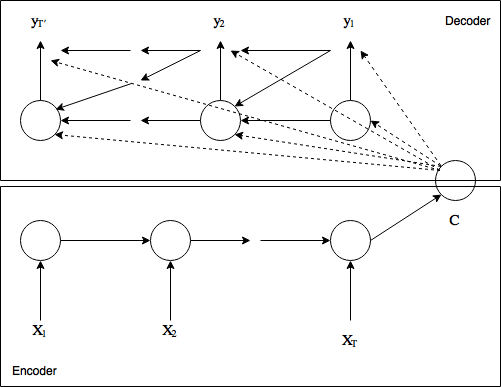
\includegraphics[width=0.8\textwidth]{fig/background_theory/encoder-decoder.png}
    \caption{An illustration of the proposed RNN Encoder-Decoder}
    \label{fig:purposed-encoder-decoder}
\end{figure}

This model, as introduced by \cite{cho2014learning}, has been used in sequence-to-sequence problems with great results. Their proposed recurrent neural network encoder-decoder model is illustrated in Figure \ref{fig:purposed-encoder-decoder}. \cite{sutskever2014sequence} proposed a similar encoder-model, but used multi-layer cells in their sequence-to-sequence model. In the description of their proposed model, \cite{sutskever2014sequence} states:

\begin{quote}
    The RNN can easily map sequences to sequences whenever the alignment between the inputs the outputs is known ahead of time. However, it is not clear how to apply an RNN to problems whose input and the output sequences have different lengths with complicated and non-monotonic relationships.
\end{quote}

The encoder-decoder model has eliminated the problem of unknown alignment between input and output. This model has therefore been found suitable for various problems with these characteristics, such as natural language processing, speech recognition, and computer vision.

\subsection{Attention Mechanism}
\label{sec:attention_mechanism}
\cite{bahdanau2014neural} conjectured that the use of a fixed-vector was a bottleneck in improving the performance of the basic encoder-decoder model. They argued that a potential issue with the encoder-decoder approach was that the neural network had to be able to compress all the necessary information of a source input into a fixed-length vector. Their proposed model extended the vector encoding by allowing the model to automatically soft-search for parts of the input to attend. With the attention mechanism, the decoder does not have to rely solely on the information in the encoded context vector, as it can supplement with information directly from the input data.

Tests of the proposed model on the task of English-to-French translation revealed that the model outperformed conventional encoder-decoder models significantly regardless of sentence length \citep{bahdanau2014neural}. \cite{bahdanau2014neural} also concluded that the attention mechanism was more robust to the length of a source sentence. Similar attention mechanisms have since then been applied to other models with improved results \citep{hsu2016recurrent, sankaran2016temporal}. 

\begin{figure}[ht]
    \centering
    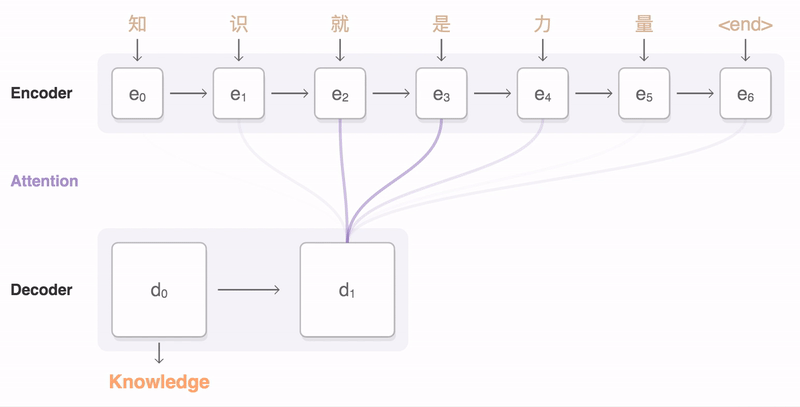
\includegraphics[width=0.8\textwidth]{fig/background_theory/attention_chinese.png}
    \caption{Encoder-decoder with an attention mechanism}
    \label{fig:encoder-decoder-attention-google}
\end{figure}

Figure \ref{fig:encoder-decoder-attention-google} illustrates a translation task between Chinese and English with an attention mechanism. The lines between the encoder and decoder indicate the degree of ``focus'' the attention mechanism pays to each part of the input. As the decoding process progresses, the area the attention mechanism attends to shifts.

%%=========================================

\section{Vocabulary Encoding}
\label{sec:vocabulary_encoding}
One-hot vectors and word embeddings are two different ways of representing a vocabulary mathematically. Vocabulary representation is necessary when working with textual data, for example in translation tasks. In this section, we look closer at pros and cons of these two encoding methods.

\subsection{One-hot vector encoding}
One-hot vector encoding is a common way to represent a vocabulary. In this encoding, we create a binary column for each unique word in the vocabulary. To represent a word we set all the binary values to \(0\) except the column that corresponds to the unique word. Table  \ref{table:one_hot_encoding} illustrates a simple one-hot encoding of a short sentence with a minimal vocabulary. 

Although this encoding method is simple and easy to implement, this approach becomes troublesome when the vocabulary is big. If the vocabulary has a total of 90,000 unique words, the one-hot vector would correspondingly need to have a size of 90,000. This vector would also consist almost exclusively of zeroes. Besides, one-hot encoded vectors neither define relationships between nearby or related words nor define any notion of semantic.

\begin{table}[H]
    \centering
    \begin{tabular}{|l|l|l|l|l|l|}
        \hline
        \textbf{Sample} & \textbf{is} & \textbf{the} & \textbf{machine} & \textbf{working} \\ \hline
        \textbf{1}      & 1           & 0            & 0                & 0                \\ \hline
        \textbf{2}      & 0           & 1            & 0                & 0                \\ \hline
        \textbf{3}      & 0           & 0            & 1                & 0                \\ \hline
        \textbf{4}      & 0           & 0            & 0                & 1                \\ \hline
    \end{tabular}
    \caption{One-hot encoding of the sentence ``is the machine working''}
    \label{table:one_hot_encoding}
\end{table}

\subsection{Word Embeddings}
An alternative to one-hot encoding is word embedding. Word embedding, also known as a type of vector space model, is a way to map vocabulary to vectors of real numbers. The concept of distributed representation for symbols dates back several decades \citep{hinton1986learning}, although the most common approaches usually follow a more modern model \citep{bengio2003neural}. The goal of word embedding is to find a representation that does not suffer from the \emph{curse of dimensionality}, problems that arise when organizing data in high-dimension space. 

The embedding is done with some parameterized function which maps the word to high-dimensional vectors. For example:

\begin{equation*}
    W(\text{"home"}) = (0.1, 0.3, 0.0, \ldots)
\end{equation*}
\begin{equation*}
    W(\text{"sun"}) = (-0.7, 0.6, 0.1, \ldots)
\end{equation*}

Usually, the \(W\) is initialized randomly, which places the words randomly in the vector space. During training of the model, the embeddings are usually trainable, and the model learns to have meaningful placement of the vectors.

Word embedding itself is a collective name for the encoding technique, and there exist different predictive models for learning word embeddings from raw data. One such model is Global Vectors for Word Presentation\footnote{\url{https://nlp.stanford.edu/projects/glove/}}, or {\tt GloVe} for short. With {\tt GloVe} embeddings, one can measure the linguistic or semantic similarity by calculating the Euclidean distance between two words.